\documentclass[letterpaper, 24pt, final, onecolumn, titlepage] {article}

\usepackage{enumerate}
\usepackage{graphicx}
\usepackage{listings}
\usepackage{color}
\usepackage{setspace}
\usepackage {amsmath}
\usepackage{amssymb}
\usepackage{verbatim}
\usepackage{afterpage}
\usepackage{geometry}
\geometry{
 a4paper,
 total={170mm,257mm},
 left=1cm,
 right=1cm,
 }

\title{ECE 270: Computer Methods in ECE \\
	\vspace{1.5cm}
   		\begin{center}\includegraphics{umlogo} \end{center}
	\vspace{1.5cm}
	\textbf{Assignment \#2} \\
	Quadratic Equation Solver}
	
\author{Hussein El-Souri}

\date{\today}

\definecolor{dkgreen}{rgb}{0,0.6,0}
\definecolor{gray}{rgb}{0.5,0.5,0.5}
\definecolor{mauve}{rgb}{0.58,0,0.82}

\lstset{frame=tb,
  language=C,
  aboveskip=3mm,
  belowskip=3mm,
  showstringspaces=false,
  columns=flexible,
  basicstyle={\small\ttfamily},
  numbers=none,
  numberstyle=\tiny\color{gray},
  keywordstyle=\color{blue},
  commentstyle=\color{dkgreen},
  stringstyle=\color{mauve},
  breaklines=true,
  breakatwhitespace=true,
  tabsize=3
}

\begin{document}

\maketitle

\doublespacing

\section{Statement of the Problem}
We need to write a program in C language that is able to solve a quadratic equation of the form $ax^2+bx+c = 0$. The program shouold be able to handle all 3 possible cases:distinct real roots, repeated real root, discrete complext roots. The result should be printed on the screen as well as into a file.\\

\pagebreak

\section{Description of Solution}
The solution for a quadratic equation yeilds two roots entirely dependant on the value of the discriminant $d$.\\
The disriminant $d$ can have three possible values each of which will give three possible solutions(combinations of roots) for the quadratic equation:
\begin{enumerate}
\item If $d>0$ the quadratic equation has two unique real solutions(roots).
\item If $d=0$ the quadratic equation has one real repeated solution(root).
\item If $d<0$ the quadratic equation has two unique complex solutions(roots).
\end{enumerate}
The numeric value for the discriminant $d$ is calculated as such:
\begin{equation}\label{discriminant}
d = b^2 -4ac
\end{equation}
And then the roots of the quadratic equation can be found through the following formula:
\begin{equation}  \label{Roots}
x_{1,2} = \frac{-b \pm \sqrt{d}}{2a}
\end{equation}
Note that in the case of $d<0$ the negative underneate the square root is dealt with as the complex number $i$ such that $i^2 = -1$.\\Then the roots are best dealt with if they are split into a real part $= \frac{-b}{2a}$ and a complex part $= i\frac{\sqrt{|d|}}{2a}$ and equation \ref{Roots} changes to:
\begin{equation} \label{ComplexRoots}
x_{1,2} = \frac{-b \pm i\sqrt{|d|}}{2a}
\end{equation}

\pagebreak

\section{Testing and Output}
The proper testing of the program is done through changing the values $a, b,\&\ c$ to cover all three possible solutions of the quadratic equation.\\
I have set the program to loop according to user input enabiling several tests the output was displayed onto a screen and into a file.\\
The screen output is placed as a screnshot on the next page (page 4).\\
The file output is imported as a text on pages 4-5

\pagebreak
\begin{center}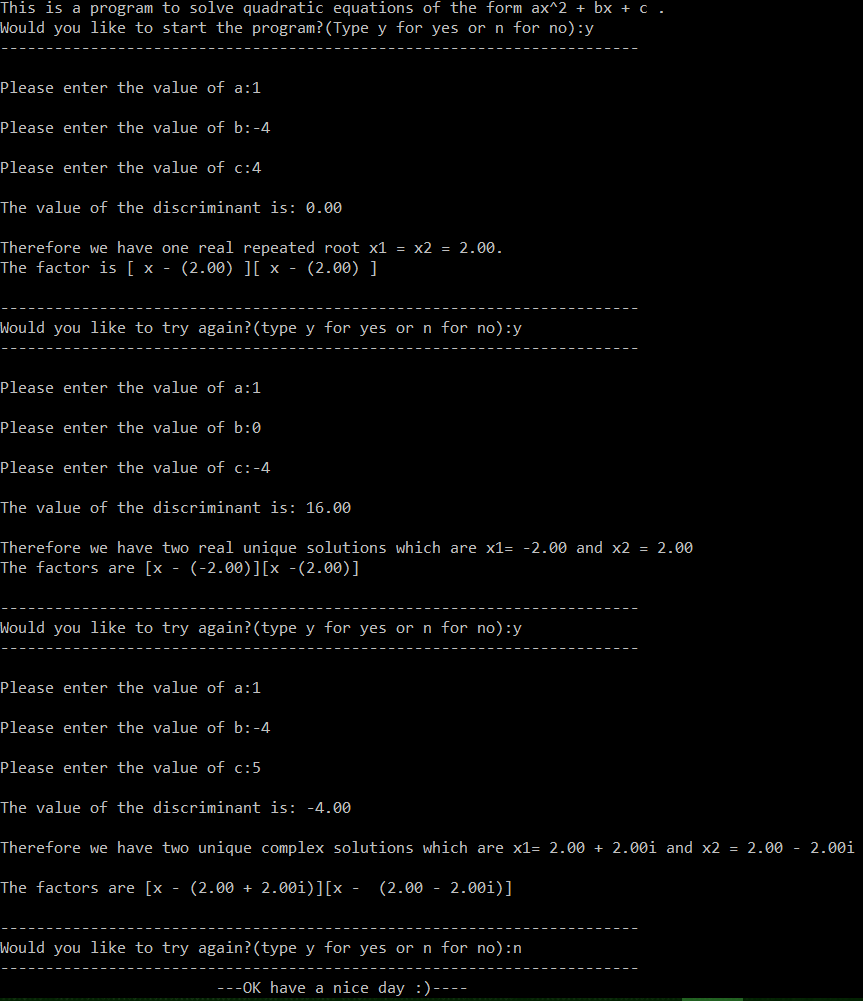
\includegraphics{output}\end{center}

\pagebreak
\verbatiminput{data.txt}
\section{Code}
\singlespacing

\begin{lstlisting}

#include <stdio.h>
#include <stdlib.h>
#include <math.h>

int main(void)
{
    //we want to create a quadratic equation solver

    float a, b, c, d,x1,x2,real,imaginary;
    char answer; //A character to introduce more user interaction through a yes/no answer
    FILE *fo;

    fo=fopen("data.txt","w");
    printf("This is a program to solve quadratic equations of the form ax^2 + bx + c .\n");
    fprintf(fo,"This is a program to solve quadratic equations of the form ax^2 + bx + c .\n");
    //----Introduction----//

    printf("Would you like to start the program?(Type y for yes or n for no):");
    scanf("%c",&answer);
    fprintf(fo,"Would you like to start the program?(Type y for yes or n for no): %c",answer);
    //---User input and interaction----//

    while(answer == 'y') //a loop to keep program running as long as user wishes//
    {
        printf("-----------------------------------------------------------------------\n");
        printf("\nPlease enter the value of a:");
        scanf("%f",&a);
        fprintf(fo,"\n-----------------------------------------------------------------------\n");
        fprintf(fo,"\nPlease enter the value of a: %.2f",a);
        //----      ----//

        printf("\nPlease enter the value of b:");
        scanf("%f",&b);
        fprintf(fo,"\nPlease enter the value of b: %.2f",b);
        //----      ----//
        printf("\nPlease enter the value of c:");
        scanf("%f",&c);
        fprintf(fo,"\nPlease enter the value of c: %.2f",c);
        //----      -----/
        d= pow(b,2) - 4*a*c; //calculating the discriminant d//
        x1= (-b-sqrt(d))/(2*a);//calculating first root//
        x2= (-b+sqrt(d))/(2*a);//calculating second root//

        //----For complex roots we have to split real part from complex part----//
        real= -b/(2*a);//calculating real part//
        imaginary= sqrt(fabs(d));//calculating imaginary part//
        printf("\nThe value of the discriminant is: %.2f\n",d);
        fprintf(fo,"\nThe value of the discriminant is: %.2f\n",d);
        if(d==0)
        {
            printf("\nTherefore we have one real repeated root x1 = x2 = %.2f." ,x1);
            printf("\nThe factor is [ x - (%.2f) ][ x - (%.2f) ]\n",x1,x2);
            printf("\n-----------------------------------------------------------------------");
            fprintf(fo,"\nTherefore we have one real repeated root x1 = x2 = %.2f and our factor is x1 + %.2f \n" ,x1,-1*x1);
            fprintf(fo,"\nThe factor is [ x - (%.2f) ][ x - (%.2f) ]\n",x1,x2);
            fprintf(fo,"\n-----------------------------------------------------------------------");
        }

        else if (d>0)
            {
                printf("\nTherefore we have two real unique solutions which are x1= %.2f and x2 = %.2f" ,x1 ,x2);
                printf("\nThe factors are [x - (%.2f)][x -(%.2f)]\n",x1 ,x2);
                printf("\n-----------------------------------------------------------------------");
                fprintf(fo,"\nTherefore we have two real unique solutions which are x1= %.2f and x2 = %.2f" ,x1 ,x2);
                fprintf(fo,"\nThe factors are [x - (%.2f)][x -(%.2f)]\n",x1 ,x2);
                fprintf(fo,"\n-----------------------------------------------------------------------");
            }
            else
            {
                printf("\nTherefore we have two unique complex solutions which are x1= %.2f + %.2fi and x2 = %.2f - %.2fi\n",real ,imaginary ,real, imaginary);
                printf("\nThe factors are [x - (%.2f + %.2fi)][x -  (%.2f - %.2fi)]\n",real ,imaginary ,real, imaginary);
                printf("\n-----------------------------------------------------------------------");
                fprintf(fo,"\nTherefore we have two unique complex solutions which are x1= %.2f + %.2fi and x2 = %.2f - %.2fi\n",real ,imaginary ,real, imaginary);
                fprintf(fo,"\nThe factors are [x - (%.2f + %.2fi)][x -  (%.2f - %.2fi)]\n",real ,imaginary ,real, imaginary);
                fprintf(fo,"\n-----------------------------------------------------------------------");
            }
            printf("\nWould you like to try again?(type y for yes or n for no):");
            scanf(" %c", &answer);
            fprintf(fo,"\nWould you like to try again?(type y for yes or n for no): %c\n",answer);
        }
    printf("-----------------------------------------------------------------------");
    printf("\n\t\t\t---OK have a nice day :)----");
    printf("\n-----------------------------------------------------------------------");
    fprintf(fo,"-----------------------------------------------------------------------");
    fprintf(fo,"\n\t\t\t---OK have a nice day :)----");
    fprintf(fo,"\n-----------------------------------------------------------------------");
    fclose(fo);
}


\end{lstlisting}

\end{document}